\section{Instrucciones}

\begin{figure}[htbp]
\begin{center}
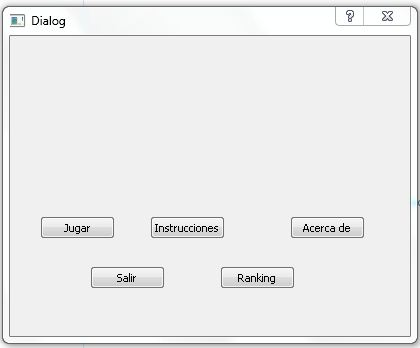
\includegraphics[width=.60\textwidth]{./imagenes/1.jpg}
\caption{Ventana Principal}
\label{Ventana Principal}
\end{center}
\end{figure}
El usuario comienza en la ventana principal, donde puede escoger cualquiera de las opciones presentadas. Para empezar el juego, le deberá dar click en jugar.


\begin{figure}[htbp]
\begin{center}
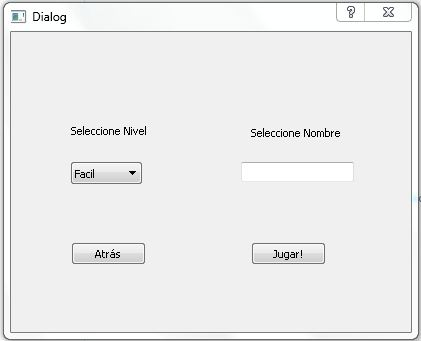
\includegraphics[width=.60\textwidth]{./imagenes/2.jpg}
\caption{Ventana de Elección}
\label{Ventana de Elección}
\end{center}
\end{figure}
En esta ventana ingresará la dificultad y el nombre. La dificultad esta dada por un número (dado por la dificultad), que al ingresar al algoritmo es el la cantidad de números que se va a extraer por recuadro.

\begin{figure}[htbp]
\begin{center}
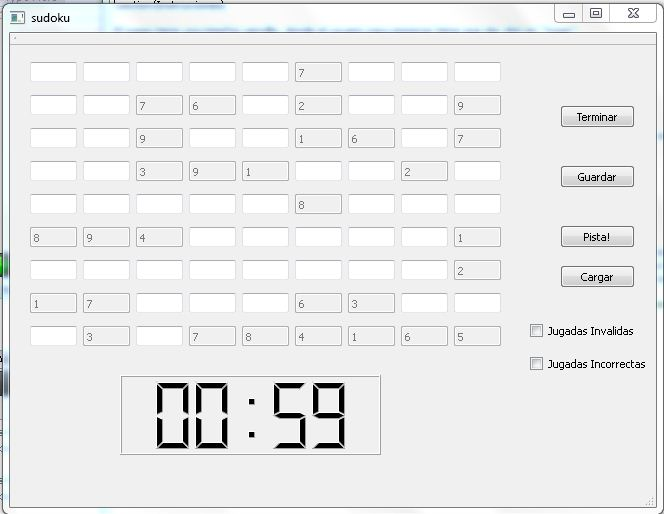
\includegraphics[width=.60\textwidth]{./imagenes/3.jpg}
\caption{Ventana del Juego}
\label{Ventana del Juego}
\end{center}
\end{figure}

Ya en esta ventana el usuario puede jugar. Se recuerda que no se podrá acceder a la funcionalidad del ranking si se carga una partida , se usa la funcionalidad pista o se usa las funcionalidades Jugadas Inválidas e Incorrectas.

Al presionar el boton pista una casilla vacía tomará el valor correcto segun la solución del sudoku.

\begin{figure}[htbp]
\begin{center}
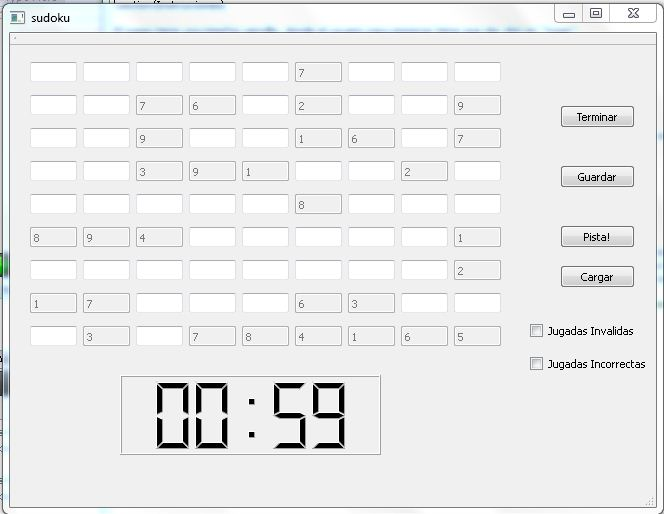
\includegraphics[width=.60\textwidth]{./imagenes/3.jpg}
\caption{Jugadas Inválidas}
\label{Jugadas Inválidas}
\end{center}
\end{figure}

Al acceder a la funcionalidad de las jugadas inválidas, se verifica el estado actual del sudoku, y jugadas incorrectas se verifica los números incorrectos con respecto a la solución del sudoku.

El reloj en la parte inferior indica el tiempo, el cuál es el puntaje del jugador.